\documentclass[12pt]{article}
\usepackage{geometry}                % See geometry.pdf to learn the layout options. There are lots.
\geometry{letterpaper}                   % ... or a4paper or a5paper or ... 
%\geometry{landscape}                % Activate for for rotated page geometry
\usepackage[parfill]{parskip}    % Activate to begin paragraphs with an empty line rather than an indent
\usepackage{graphicx}
\usepackage{amssymb}
\usepackage{epstopdf}
\DeclareGraphicsRule{.tif}{png}{.png}{`convert #1 `dirname #1`/`basename #1 .tif`.png}

\title{Engineering Ethics -- An Essay to Accompany Presentation}
\author{Theodore G. Cleveland, Ph.D., P.E.\\}
\date{17 October 2006}                                           % Activate to display a given date or no date

\begin{document}
\maketitle
\section*{Introduction}
Ethics is the study and practice of principles that govern activities between people in their personal and professional lives.  Professional ethics are principles that govern activities between professionals and their clients, customers, and the public.  Engineering ethics includes the general concepts of professional ethics but also includes principles governing activities related to the approval of plans, designs, specifications and requisite qualifications (of engineers).

Ethics and the concern regarding their importance to society have been around as long as there has been society.  Most ethical principles have evolved from centuries of human experience and are common to all cultures.

Examination of the ''definitions'' above contain two important components; 
\begin{enumerate}
\item principles that govern activities provide guidance for how we act.
\item requisite qualifications provide guidance for whom should act.
\end{enumerate}

The remainder of this article discusses some principles relevant to engineering ethics in today's society.  Although the article appears to be authoritative, it is not\footnote{This essay and the presentation contain copyrighted materials, it is the authors' opinion that use of these materials is within the fair-use provision of U.S. Copyright law, however any redistribution of these materials outside the course would materially violate U.S. Copyright law.}.  I am not a licensed lawyer, or credentialed philosopher (although I suppose the Ph.D. might count).  I have tried in good faith to acknowledge where I obtained the thoughts and opinions presented in this article, but few parts are truly my own work.  This article should be read with that understanding; the references to parts of the Texas Engineering Practices Act may have moved around, and the reader is expected to seek out the appropriate sections of the Act to understand the ethical implications expressed in the Act.

\newpage
\section*{Philosophical Perspective}
Ethics is not a new concept.  While the ``study'' has been around since the dawn of society, the topic was recently formalized in Western thought in the 1700's.  At this time in history, the divine right of kings was successfully challenged and popular governance emerged.  The philosophers of the times examined ethics at the time, because popular governance changed the concept of ''noblese obligee'' or noble obligation and everyone had to assume the responsibility for a decent society.\footnote{ The responsibility was always shared among everyone, but when monarchies, failed the effort was somewhat redistributed}

\subsection*{Ethical Theories}
The philosophers of this time period identified several ways of ethical reasoning, or moral models of behavior.  Condensed into three categories these are (in no particular order): value, duty, and utility theories.

\begin{enumerate}

\item Value ethics are ethics based on the moral concept of virtue.  This mode of reasoning is focused on the ''character'' of the individual. Correct behavior (virtue) are actions that lead to or stem from ''good'' character traits.  Incorrect behavior (vice) are actions that lead to or stem from bad character traits.
Society defines ''virtue'' and ''vice.''  All cultures from the most primitive to the most advanced have uniformly common concepts of ''good'' and ''bad'' \textbf{character}. \footnote{Character is different from particular behavior.  Corruption is perceived differently in different parts of the world (Brown, 2004), but good character is essentially uniform.}

\item Duty ethics are ethics based on the moral concept of duty.  Ethical behavior is a set of fundamental duties for which  all citizens are responsible (Immanuel Kant 1724-1804).  An intimately related concept is the concept of individual rights.  Individuals have certain rights that are to be respected (John Locke, 1632-1704) by others (e.g. life, liberty, property, etc.).\footnote{Notice the date of Locke's work.  Thomas Jefferson borrowed nearly verbatim in the declaration of independence for the United States.}  So to summarize these thoughts,  ethical behavior is a duty, and our duty is to uphold certain individual and collective rights.  Some parts of the Texas Engineering Practices Act describe the engineer's duties to society and each other.  These components clearly trace their origin to the concept of duty ethics that was formalized in Kant's writings. 

\item Utility ethics are ethics based on the moral concept of what is good for \textbf{society}.  This category of reasoning extends past the individual and attempts to develop structures for society as a whole to operate. Actions that maximize well being of society are the goal of this type of ethical thought.
Utility, usefulness, and benefit are all fundamental ideas in this mode of ethical reasoning.  An important concept is that benefit or well being of the \textsl{individual} may be subservient to well being of society.

John Stuart Mill (1806-1873) struggled with how to combine the concepts of utility ethics with the other models of behavior that focused on individual behavior.  His concept of act utilitarianism focused on actions.  He argued that  individual actions should be judged based on whether the most good was produced (for society), and rules should be broken if doing so will lead to the most good.  A logical criticism of his argument is that it begs definition of ''good.''  

The argument of utility is frequently hijacked by tyrants who would use Mill's logic to justify atrocious behavior if the outcome is presumably good.  Machiavelli recognized in a different context the same moral flaw in his concept of  ''The end justifies the means.''   Machiavelli's  writings were a guide book for taking and maintaining power in a world of small principalities (monarchies).  

I would argue that Mill's never intended the idea to be corrupted by tyrants, but more along the lines of ''The needs of the many outweigh the needs of a few.''  This quote is from Spock, a character in the original  Star Trek series.  I doubt it is original, but it is an eloquent statement of the guiding principles of utility ethics.  Usually (in the TV show) after this statement, an entire planet would be on the verge of destruction unless a few individuals would sacrifice themselves into fictional oblivion.  On the show, the sacrifice only went so far as willingness, and at the end the planet was saved and no one was hurt. \footnote{American Television's  lack of appreciation for tragedy is why the outcomes were usually benign -- but then again, tragedy does not sell beer and soap}.  Obviously the series was ''space opera'' but the writers did have a sense of literature and identified that entertainment could have impact on thought.

Common rules of morality (do not steal, do not harm others, be honest, etc.) are consistent with this concept and are guidelines developed from centuries of human experience.  Sometimes these common rules must be violated to achieve common benefit. (e.g. it might be justifiable to steal food to prevent starvation).\footnote{I developed this article well before Hurricane Katrina. But as an example of utility ethics people who broke into Wal-Mart and stole food, water, and medicine for their own \textbf{immediate} survival were morally justified in that instance (it was still illegal).  However, those who stole TVs, radios, clothes, liquor etc. --  items totally unrelated to survival were wrong!}

A subset of utility theory is a concept called rule utilitarianism.  Rule utilitarianism is focused on compliance.  This theory holds that sacrifice in certain situations to uphold \textbf{rules} ultimately leads to the most good.  One of the difficulties is that it presumes that the rules are correct.  Most certainly are, but in some circumstances, adherence to rules creates a dilemma.  Figure 1 is a humorous perspective on morality and its relationship to a dilemma. 
 
\begin{figure}[h!] %  figure placement: here, top, bottom, or page
   \centering
   \includegraphics[width=3in]{./figures/CarlsDilemma.pdf} 
   \caption{Carl's dilemma -- Actually not a true dilemma, Carl has a third but in-obvious choice - he could carry the pirate to safety!}
   \label{fig:example}
\end{figure}

For instance if the rule is unjust, but everyone is forced to comply, then one can make the argument that
an unjust rule applied uniformly is fair.  However, the argument holds only if everyone is treated the same; otherwise we end up in the Orwellian situation that ''All pigs are equal, but some pigs are more equal than others.''  In practice rules are not applied uniformly, and thus dilemmas are common.  Taken to the extreme compliance might do more harm than good (consider the Katrina example regarding immediate survival)

\item Finally, benefit-cost analysis is fundamentally an application of utilitarianism. Costs of an action are usually straightforward to predict. Benefits require guess work; some benefits are not economically quantifiable.

Often only policy (politics) can assign benefit in these situations.  Like the more abstract points above, the question always arises (think of the pigs) \textsl{Are those who benefit the same as those who bear the costs?}  Consider taxation and public infrastructure - some fraction of our taxes goes to benefit people in South Dakota - how much benefit do we (bearing a portion the cost) receive?  Of course, they pay taxes that we spend, so there is at least in concept, some economic parity.
\end{enumerate}

So what is the point?  The point is that ethics is neither new nor well posed - there will always be conflicts and that is the purpose of the ethics component of continuing education.  The real goal is to identify when conflicts exist and provide us with a way to reason through them, and that reasoning needs to be based on value, duty, and utility and not just economic gain.  Also notice in the theories the unifying concepts of ''virtue'' and ''individual and common good.''

\newpage
\section*{Bribery, Corruption, and Corporations}
The apparently recent emphasis of ethics in engineering arises from recognition and collective desire to combat bribery and corruption in engineering projects.   The consensus that bribery and corruption is unacceptable is not just based on moral arguments but is thought to consume about 3\% of the gross domestic product of the entire world, about 5 trillion dollars globally or about \$900 per person on the planet\footnote{ http://en.wikipedia.org/wiki/Image:World GDP Capita1-2003 A.D.png ; I assumed 6 billion world population}. 

Figure~\ref{fig:soul_for_a_donut} is a humorous view of the moral transaction of corruption and bribery.  Wally being of little character sells his soul for a donut!

\begin{figure}[h!] %  figure placement: here, top, bottom, or page
   \centering
   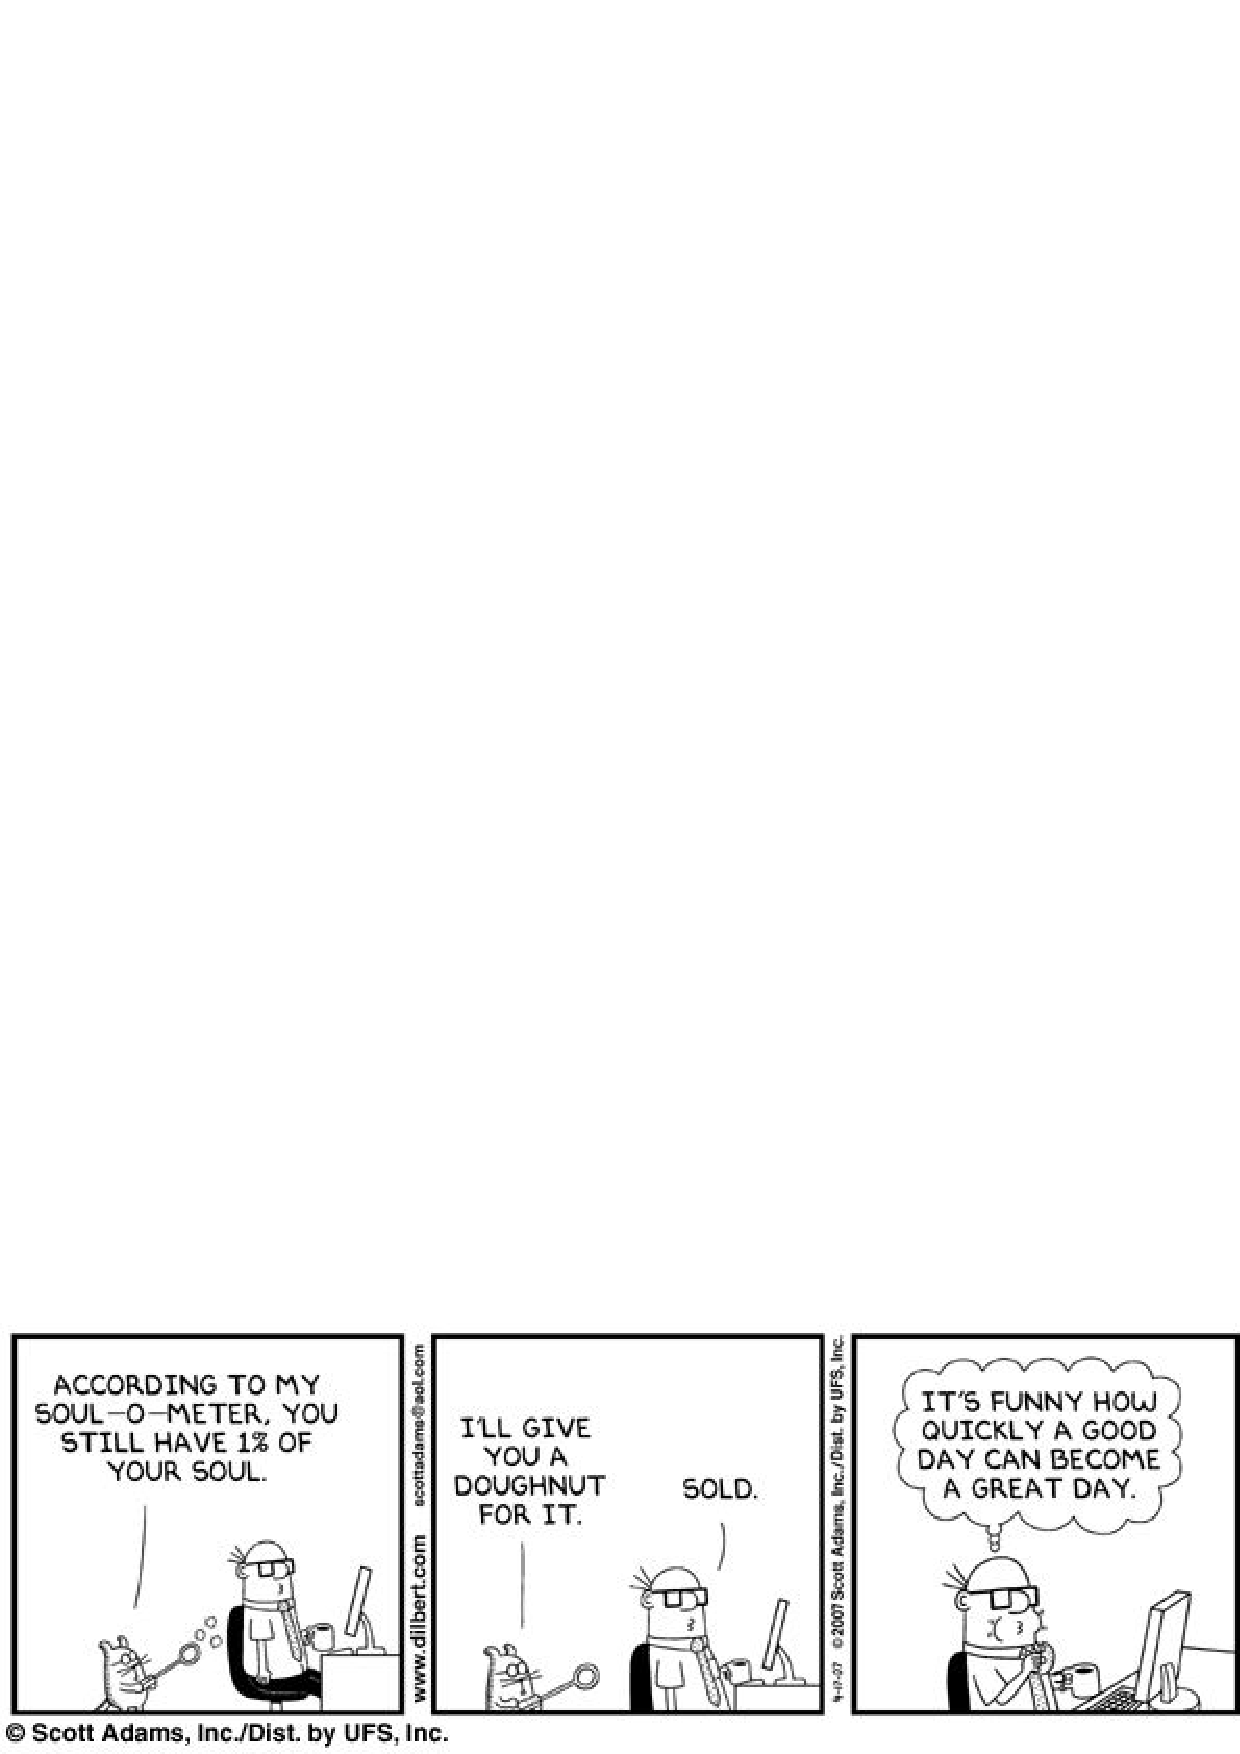
\includegraphics[width=4in]{./figures/soul_for_a_donut.pdf} 
   \caption{Wally sells his soul for a donut; corruption costs a lot more than donuts, but is essentially the same transaction.}
   \label{fig:soul_for_a_donut}
\end{figure}

From an economic argument alone, ethics (which is probably the only tool that can fight corruption - I argue that briefly a little bit later) is worth frequent examination.  Most firms are doing their best to define and implement anti-corruption policies, but many lack consistency, fail to collect feedback, and fail to recognize acts of integrity as well as acts of corruption.   If integrity is not actively recognized in some meaningful fashion, policies do little good.  As an example, the U.S. Congress has a Code of Ethics, but if members don't bother to follow the code, and Congress fails to self-police, then the code is just wasted paper (The readers can make "jokes" at the expense of Congress at their leisure!). 

There is considerable lack of enforcement worldwide often because of a subtle but important distinction between legal and ethical behavior.  One common theme often cited is that corruption is perceived differently in various parts of the world, and thus a universally accepted code of conduct would be difficult because cultural differences conspire against a uniform view of corruption.  This statement may be true in a legal context, but in an ethical context I argue the opposite; Ethics provides considerable clarity.  Virtue, duty, and utility are uniform principles regardless of culture - and that is likely why the emphasis on ethics is so important in engineering. \footnote{Most of this section is based on an article by Jeff Brown in the November 2004 ASCE News.}

Relevant to this discussion is the corporate mentality regarding morality.  In principle, a corporation is not a person, hence it cannot be a moral agent.  Because it is not a moral agent, corporations can neither be ethical nor unethical.  However, corporations are comprised of people and deal with people.
Because of these interactions with people, corporations are expected to behave morally, even though it is unenforceable (in the legal sense). 

\newpage
\section*{Ethics and Law}
Notice in the last section there was the mention of enforcement in the discussion on bribery and corruption.  This issue begs a brief discussion of an important difference between law and ethics.  Law, or more precisely legal behavior, is behavior and conduct and actions that are in agreement with codified (written) standards in some legal documents by some appointed \footnote{The method of appointment is irrelevant, the legal body can be directly elected, appointed, or self-appointed, although the latter method might meet considerable resistance in the USA} 
legal body; those documents and the legal experts together determine what is law and whom should obey it.  The key points are that law is codified(written), interpreted by a legal body (the courts), the
documents and the legal body determines what is legal, and \textbf{may not apply to all}.

Figure   \ref{fig:ethics_and_law} presents a popular perception of ethical and legal behavior -- no doubt reinforced by the news media's coverage of congressional ethics.    There is probably some element truth to the dilemma proposed by the comic strip, but in business situations, such a dichotomy of behavior is probably rare.

\begin{figure}[ht!] %  figure placement: here, top, bottom, or page
   \centering
   \includegraphics[width=3in]{./figures/ethics_and_law.pdf} 
   \caption{A popular view of ethics and law as it pertains to business; that is they are diametrically opposed.}
   \label{fig:ethics_and_law}
\end{figure}

Ethics, or more precisely ethical behavior, is behavior and conduct and actions that lead to outcomes that are socially acceptable (beneficial) and do not unduly impact individual rights.  In contrast to legal behavior, ethical behavior is defined by society, not necessarily written, exists independently of any ''experts,'' and applies to all members of society.  The distinction is subtle but important - things that are unethical are not necessarily illegal.  The converse is probably also true in some instances.  This brings us to the important part of the seminar, which are tools for making ethical choices.
\begin{figure}[ht!] %  figure placement: here, top, bottom, or page
   \centering
   \includegraphics[width=3in]{./figures/ethics_or_business.pdf} 
   \caption{Another view of business principles (policy) and ethics; notice both doors go to the same place.}
   \label{fig:ethics_or_business}
\end{figure}
Figure  \ref{fig:ethics_or_business} is an alternate view of business and ethical behavior, and is probably a more meaningful allegory.  Both doors enter into the same place, the ethical door is smaller and requires far greater effort to squeeze through, while the policy door is huge.
\newpage
\section*{Making Ethical Choices}
The most important tool for making ethical choices is between the ears, and depends on personal commitment to good character.  The rigor of an engineering education generally selects out the truly unethical - so this section is really geared for handling the dilemma - the situation where both courses of action require some kind of compromise and potential damage. 

The general guiding principle is choices are to be based on engineering ethical standards above personal standards. All the engineering professional societies have Codes of Ethics to guide the decision, and the Texas Engineering Practices Act's section on ethics also provides a guide.  We will study parts of the act shortly.  Figure~\ref{fig:drZook} is a humorous perspective on medicine and its relationship to society.  The medical profession's mission is the amelioration of injury and illness; they expect to be paid, but even though physicians directly advertise I suspect that the soldier's shock is about the "in-your face" nature of Dr. Zook's approach.  The point of the figure in this seminar is that ethics is a concern in our daily lives.

\begin{figure}[ht!] %  figure placement: here, top, bottom, or page
   \centering
   \includegraphics[width=5in]{./figures/DrZook.pdf} 
   \caption{Dr. Zook's advertising - at one time the medical profession thought that advertising was an unprofessional and tasteless business practice; that thought has changed.  Dr. Zook appears to be opportunistic, and I suspect the cartoonist intended the allegorical tone.}
   \label{fig:drZook}
\end{figure}

Figure~\ref{fig:poop_on_car_ethics} is a similar example of ``in-your-face'' promotion of a business.  The engineering equivalent would be to damage public structures to obtain engineering services, or to intentionally design shortened life spans of engineered things, planned obsolesce is common in product engineering, but should never be part of a system engineered for the public.  Planned obsolesce is not the same as things wearing out and needing maintenance and replacement -- but if a choice is made for the purpose of additional business it is probably unethical.

\begin{figure}[h!] %  figure placement: here, top, bottom, or page
   \centering
   \includegraphics[width=3in]{./figures/Poop_on_car_ethics.pdf} 
   \caption{Guerilla advertising; engineering equivalent is planned obsolesce in order to obtain future work.}
   \label{fig:poop_on_car_ethics}
\end{figure}

\subsection*{A Fable}
These issues are quite timeless.  Consider fables.  Fables are very simple allegorical stories originally invented as a form of political criticism and as a tool to teach cultural values.
One such fable is that of Mercury and the Woodcutter.

\begin{em}
"A Woodsman was felling a tree on the bank of a river, when his axe, glancing off the
trunk, flew out of his hands and fell into the water. As he stood by the water's edge
lamenting his loss, Mercury appeared and asked him the reason for his grief. On learning
what had happened, out of pity for his distress, Mercury dived into the river and, bringing
up a golden axe, asked him if that was the one he had lost. The Woodman replied that it
was not, and Mercury then dived a second time, and, bringing up a silver axe, asked if
that was his. "No, that is not mine either," said the Woodman. Once more Mercury dived
into the river, and brought up the missing axe. The Woodman was overjoyed at
recovering his property, and thanked his benefactor warmly; and the latter was so pleased
with his honesty that he made him a present of the other two axes. When the Woodman
told the story to his companions, one of these was filled with envy of his good fortune
and determined to try his luck for himself. So he went and began to fell a tree at the edge
of the river, and presently contrived to let his axe drop into the water. Mercury appeared
as before, and, on learning that his axe had fallen in, he dived and brought up a golden
axe, as he had done on the previous occasion. Without waiting to be asked whether it was
his or not, the fellow cried, "That's mine, that's mine," and stretched out his hand eagerly
for the prize: but Mercury was so disgusted at his dishonesty that he not only declined to
give him the golden axe, but also refused to recover for him the one he had let fall into
the stream."
\end{em}

Let us ask ourselves some simple questions about the fable.
\begin{enumerate}
\item What is the �moral� or lesson of this fable?
\item Does this fable have any relationship to ethical situations (of course, but what?)
\item What were the consequences of the second woodsman�s �unethical� behavior?
\end{enumerate}

To summarize to this point.  Ethics is crucial to how engineers do their jobs; there is a compelling economic argument for ethical behavior in the context of corruption; and the issue is timeless - it plagued ancient people as well as ourselves; and finally, ethical theories suggest that there will, at times, be conflicts or dilemmas and some reasoning tool is needed to select a subsequent action.   The fable itself is the ancient equivalent of today's codes of ethics -- it was intended to guide people into making ethical (and civilized) choices.

Why a code of ethics?   By analogy consider that soldiers, police, firefighters, EMTs etc. are expected to perform in very high-stress situations with practically no time to think.  In their work, they endure nearly continuous training to function in a manner to ensure high-probability of correct response.   If patterns of failure are detected, the training is changed.  Code of ethics serves a similar purpose.
The codes provide guides to behave to an ethical issue (dilemma) in a manner to ensure a high-probability of correct response.

The National Society of Professional Engineers (NSPE) is one example of a code of ethics.  The discipline specific codes of ethics are essentially clones of the NSPE code.  The ethics section of the Texas Engineering Practices Act is also a nearly verbatim copy of the NSPE act - except that since the Act is legislation, it does have the force of "law" behind it - in essence an unethical practice of engineering in Texas is also illegal.

\section*{NSPE Code of Ethics}
The NSPE code of ethics is actually pretty simple in structure.  There is the preamble that describes the purpose of the code which is to safeguard life, health, property,\footnote{Duty Ethics} promote the public good, \footnote{Utility Ethics} and maintain high integrity\footnote{Value Ethics - I am assuming that the NSPE is focused on the individual engineer's character - recall that to be licensed one question that our SER reviewers must answer is if they think the candidate is moral enough to be an engineer - a question of character.}.

The next part of the code is the fundamental canons.  These are simply a set of rules that engineers are expected to follow.  The rules deal with only three fundamental issues: Engineers are obligated to uphold public welfare, obligated to be competent, and are obligated to be honest.  The individual rules paraphrased are:
\begin{enumerate}
\item  Public welfare is paramount.\footnote{Like the "prime directive" in the Star Trek series.} The code provides guidelines for how to act in generalized situations.  It describes correct engineering behavior.  Notes that engineers have an obligation to report illegal and unethical behavior.
\item Obligated to work in areas of competence.  Both the NSPE code and the Texas Engineering Practices Act observe that experience and/or education confers �competence�.  Self-education would qualify (hard to prove).  Judgment is expected.  Project management is covered (modern management theory).  
\item Tell the truth; Requires disclosure if paid for an opinion (in advance of the opinion). 
\item Preserve the engineer-client privilege (confidence, secrecy, competitive advantage).  Disclose conflict of interests -- esp. applies to public employees.
\item Be honest; Respect other engineers.  Do not misrepresent ones own abilities or downplay a competitors abilities.  This rule does not preclude pointing out a competitors experience (which is a matter of business records), but one truly has no way of determining a competitors ability.  Don�t accept things that are or look like a bribe, kickback, payoff etc. to obtain a job.  You can still meet with your friends for lunch, discuss work, and even take turns paying the bill.  
\item Uphold your obligation to the profession.  One obligation is to teach others - thus that competitive advantage above eventually should be shared.  Oddly enough improving your competitors capabilities not only promotes the public good, it is probably good business in the long run.  
\end{enumerate}

\section*{Texas Engineering Practices Act}
The act is fairly long 70 or so pages.  The ethics and professional development component is a small but important part of the Act.  A majority of the Act establishes legislative authority, how it is funded, etc.  The important parts for this seminar are that the Act defines the ''practice of engineering'', defines ''licensure qualifications'' and defines ''misconduct.''  Some of the relevant sections for this seminar are listed below.

\S 1001.004 Establishes the purpose of the Act:  Promote the public good, improve quality of life, property, economy, and security of the state and the nation.

\S 1001.$...$ Specific definitions; defines a public work, sets dollar values on projects that need licensed engineers to perform services; establishes fees for various license related activities.

\S 1001.210 Establishes the continuing education program - this seminar is relevant in the context of this section.  The continuing education component is generous - there is no reason why a person cannot accumulate the required annual development hours the things that count include:

\begin{enumerate}
\item A course sponsored by an institution of higher education, a professional, or a trade organization
\item A seminar, tutorial, short course, correspondence course, videotaped course, or televised course.
\item Participating in an in-house course sponsored by a corporation or other business entity
\item Teaching a course described by the Act
\item Publishing an article, paper, or book on the practice of engineering
\item Making or attending a presentation at a meeting of a technical or engineering management society or organization or  writing a paper presented at such a meeting; 
\item Participating in the activities of a professional society or association, including serving on a committee of the organization
\item Engaging in self-directed study (up to 5 hours).
\end{enumerate}

At least 1 hour needs to be ethics related, reading the act each year would count and could be logged in the self-directed component.

\S 1001.301. A license is required to practice engineering and/or use following titles: 
\begin{enumerate}
\item engineer
\item professional engineer
\item licensed engineer
\item registered engineer
\item registered professional engineer
\item licensed professional engineer
\item engineered ... (used as verb/adverb?) in describing some work.  This particular word is in that grey area - my laptop is engineered, but I am sure the State of Texas had no say in who, where, or how.  On the other hand my sewage collection system was engineered and that was well within the provisions of the act.
\end{enumerate}

The next section delegates state authority to political subdivisions of the state.

\S 1001.402. Enforcement by Certain Public Officials.
A public official of the state or of a political subdivision of the state who is responsible for enforcing laws that affect the practice of engineering may accept a plan, specification, or other related document only if the plan, specification, or other document was prepared by an engineer, as evidenced by the engineer�s seal. 

The next section deals with engineering requirements for a public work where consequences involve health, welfare, and safety.

\S 1001.407. Construction of Certain Public Works 
The state or a political subdivision of the state may not construct a public work involving engineering in which the public health, welfare, or safety is involved, unless: 

(1) the engineering plans, specifications, and estimates have been prepared by an engineer; and 

(2) the engineering construction is to be performed under the direct supervision of an engineer. 

The next section contains detailed definitions of various items - of particular interest is negligence and incompetence.

\S131.81 Definitions
Defines meanings of acronyms (ABET) etc. and specific terms such as �graduate engineer� etc. 

Gross negligence - Any \textbf{willful} or \textbf{knowing conduct}, or pattern of conduct, which includes but is not limited to conduct that demonstrates a \textbf{disregard} or indifference to the \textbf{rights}, \textbf{health, safety, welfare, and property} of the public or clients. 

Gross negligence \textbf{may} result in financial loss, injury or damage to life or property, but such results \textbf{need not occur} for the establishment of such conduct. 

This last sentence means that "no harm no foul" is not a defense.

Incompetence - An \textbf{act} or \textbf{omission} of malpractice which may include but is not limited to \textbf{recklessness} or \textbf{excessive errors}, omissions or failures in the license holder�s record of professional practice; or an act or omission in connection with a disability which includes but is not limited to mental or physical disability or addiction to alcohol or drugs as to \textbf{endanger} health, safety and interest of \textbf{the public} by impairing skill and care in the provision of professional services. 

The quote "Don't drink and derive" has more significance than a funny pun on a t-shirt.

Summary: Negligence is disregard for rights, safety, etc.   Harm need not occur for negligence.  Incompetence is recklessness, inability, impaired or missing skill that endangers the public - notice that the first part includes poor record keeping (that endangers the public).   Also observe that the words explicitly acknowledge that engineers may make mistakes - it demands that there be few of these and that we behave in good faith.  Engineering involves risk of failure and advancement of the state of knowledge may indeed lead to failure - the Act (in my opinion) acknowledges such and simply demands that engineers do not willfully disregard safety, keep good enough records so we (the profession) can learn from mistakes, and that we do not make too many at once.

\S137.37 Sealing Misconduct.  A license holder shall be guilty of misconduct and subject to disciplinary action if the license holder: 

(1) knowingly signs or seals any engineering document or product if its use or implementation may endanger the health, safety, property or welfare of the public.

(2) signs or affixes a seal on any document or product when the license is inactive or has been revoked, suspended, or has expired. 

(3) alters a sealed document without proper notification to the responsible license holder.

The last part of this section of the seminar lists the some of the section titles of the ethics section of the Act.  If you compare these to the NSPE code of ethics the parallel is obvious (order is different!).

\S137.55 Engineers Shall Protect the Public

\S137.57 Engineers Shall be Objective and Truthful

\S137.59 Engineers� Actions Shall Be Competent

\S137.61 Engineers Shall Maintain Confidentiality of Clients 

\S137.63 Engineers� Responsibility to the Profession

\section*{Documentation of Professional Development}
Documentation is simple, and important.  I know of several people who have been audited, and it appears that the board intends to audit a sample of all licensed engineers every year.    The Act specifies that the engineer should maintain a log of professional development activities as well as proof of those activities in the form of completion certificates and so forth.  The TBPE has an on-line log tool you can use, a paper based log, and I suppose even a calendar entry would be sufficient.  The minimum information the act expects you to be able to provide are type of activity, sponsoring organization, location, duration, instructors name, and PDH credits claimed.  

If you are audited, and the board decides the activities are insufficient the Act specifies that the board may require the license holder to obtain the requisite hours as needed in activities that meet the board's approval.

\section*{Bibliography}
This article was written using materials cited in footnotes as well as the following materials

Brown, Jeff. 2004. "Workshop advances global principles of professional conduct" ASCE News November 2004.

Fleddermann, C.B., 1999. Engineering Ethics. Prentice Hall, NJ 135p.

Potter, M.C., 1999. Fundamentals of Engineering (FE Review Book). Great Lakes Press, Okemos, MI. 627p.

Texas Engineering Practices Act (on web - google texas Board of Professional Engineers  for a current copy).

Locke, John. 1689. Two treatises of government   (in public domain).  This document is a likely source of much of Jefferson's thoughts.

Locke, John, 1689. An essay concerning human understanding   (in public domain).

Mill, John Stuart. 1859.  On Liberty (in public domain).

Mill, John Stuart. 1861. Utilitarianism (in public domain).

Kant, Immanuel. 1785.  Grundlegung zur Metaphysik der Sitten (Grounding for the Metaphysics of Morals) (in public domain).

Kant, Immanuel. 1788.  Kritik der practischen Vernunft (Critique of Practical Reason) (in public domain).



\end{document}   